\documentclass{article}
\usepackage{graphicx}
\usepackage[utf8]{inputenc}
\usepackage[margin= 3.5cm, includefoot]{geometry}
\usepackage{caption}
\usepackage{subcaption}
\usepackage{amsmath}
\usepackage{mathtools}
\usepackage{float}
\usepackage{verbatim}
\usepackage{ulem}

\title{Mind Your Hinglish}
\author{\hspace{0.55cm}Aniket Gupta\hspace{2cm}Aayush Goyal\hspace{2cm}Anshuman Panda\\2019CS10327\hspace{2.2cm}2019CS10452\hspace{2.4cm}2019CS10463}

\date{October-November 2021}

\begin{document}

\maketitle

\section{Introduction}
Were you taught Hindi in your school? What about English? Have you ever thought ki inn dono mein se zyada frequently tum konsi language use krte ho? And did you just realize that the former line contains morphemes of both Hindi and English? Do you know this mixing of Hindi and English has got \sout{official} name called Hinglish? Most of the academic curicullums frown upon mixing of Hindi and English, so here we will be discussing more on the depths and breadths of Hinglish.
\\\\
Hinglish, the language used by most of the Indian natives nowadays is a blend of both Hindi and English. It is a macaronic use of English with Hindi morphemes involving code switching and code mixing between these languages where they are freely interchanged according to the ease of use. This is widely in use because of the ease of speaking and writing. Mostly the people are not very frequent in using English and nor are they very proficient in pure Hindi and hence are observed to use a mix of these both, that is, Hinglish. Such code mixing and code switching has crept it's way into advertisements, newspapers, magazines, TV shows, Bollywood movies as well as the corridors of political and corporate powers in India. 
% TODO: write some survey about the ease of use between these thre laanguages. 
\\\\
Have you ever thought about how did Hinglish came to be? Have you ever thought how it became the language of the common even if it is not taught in any school and curicullum? Even the poeple who have not received any formal education in any of these 2 languages are seen using it in their daily life. How long do you think Hinglish has been in existence? Is it limited to the modern Indian youth influenced by the social media platforms? or it has been in existence much before the social media platforms became popular? What all do you think has given rise to the rapid growth in popularity of hinglish? Is it limited to the "upper-class elite" Indians or is it used in the semi-urban and the rural centres as well? 

\section{Rise of Hinglish}
It is a general misconception that this language has came into existence because of the influence of modern social media platforms and internet on the modern Indian elite class groups. In fact the use of hinglish can be traced back to time when India was under british rule. The british government at that time used english but most of the Indian were not good in English. These interaction of english and hindi speakers led to the use of words of both the languages to some extent by both sides, the government and the people. The example of use of hinglish, during the british rule can be observed in the words of Ayodhya Prasad Khatri (1857-1905), a prominent hindi poet. He wrote:
\begin{quote}
    \centering
    \textit{Rent Law ka gham karen ya Bill of Income Tax ka?\\
    Kya karen apan nahiin hai sense right now-a-days.\\Darkness chhaaya hua hai Hind men chaaro taraf\\
    Naam ki bhi hai nahiin baaqi na light now-a-days.}
\end{quote} 


\section{Social Media Influence}


\section{Usage and Popularity among the people}
Given the increasing use of Hinglish in the modern world, we have gathered some results of the surveys on how indians prefer HInglish over Hindi and English. In this we have analysed the usage and popularity of Hinglish among the people from different age groups, regions and class of people. The survey conisited of 744 people and we have made 4 different categories to which the people belong to. The categories are as follows:
\begin{enumerate}
    \item \textbf{Age Group:} The age group to which they belong to.
    \item \textbf{Origin Factors:} The region to which they belong to.
    \item \textbf{Mother Tongue:} The mother tongue to which they belong to.
    \item \textbf{Frequent Usage:} The frequency of use of which Language by the people.
\end{enumerate}
And further in all of these groups we have focused on 4 aspects of usage and popularity of Hinglish. The 4 aspects are as follows:

\begin{enumerate}
    \item \textbf{Mixing of Languages:} How often use Hindi and English by mxing them, ie, as Hinglish.
    \item \textbf{Speed of Reading:} How fast the people read the Hinglish written in the Latin script (basically using words from English) rather than in the Devnagari script.
    \item \textbf{Preferred Script:} Which script is preferred by the people to read and write the Hinglish language, whether in the Devnagari script or the Latin script.
    \item \textbf{Exposure to Hinglish:} How much are they exposed to Hinglish.
\end{enumerate}
Below is the analysis of different aspects of Hinglish for each group as stated above.

\subsection{Age Group}
The age groups can be broadly into the following categories:
\begin{enumerate}
    \item \textbf{Gen X:} People who are 44 and older. This is about 36.2\% of the respondents of survey.
    \item \textbf{Gen Y:} People who are 25 to 44. This is about 44.2\% of the respondents of survey.
    \item \textbf{Gen Z:} People who are 15 to 24. This is about 19.6\% of the respondents of survey.
\end{enumerate}
A detailed distribution of people belonging to different age groups is in the figure below:
\begin{figure}[H]
    \centering
    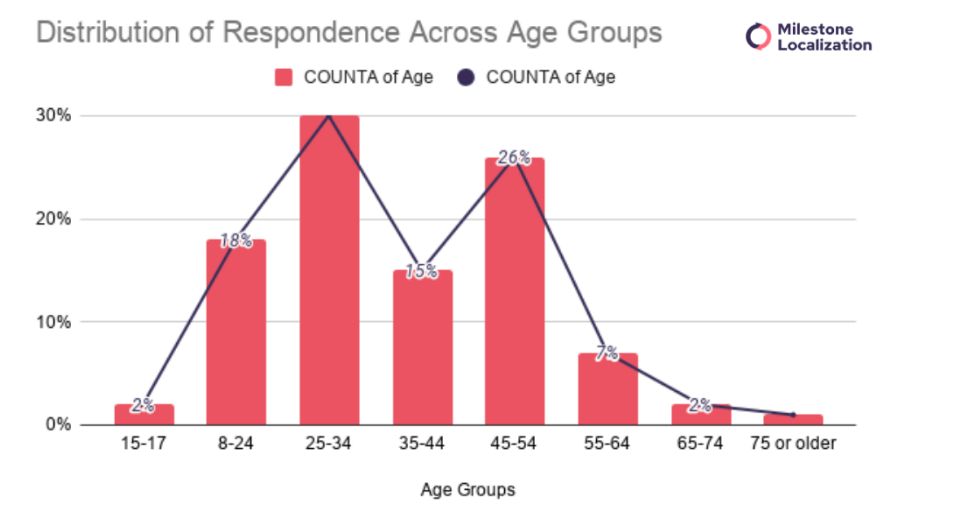
\includegraphics[width=0.8\textwidth]{plots/distribution_with_age.png}
\end{figure}

\subsubsection{Mixing of Languages}

\begin{figure}[H]
    \centering
    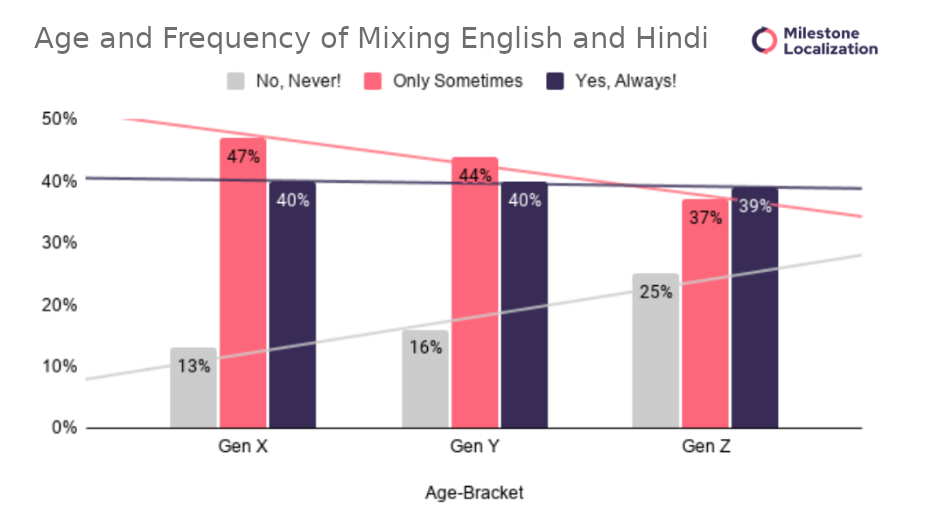
\includegraphics[width=0.8\textwidth]{plots/age_mixing_language.png}
\end{figure}
From the above it can be inferred that the people who are in the age group Gen X are more likely to use Hinglish than the people in the age group Gen Y and Z. As we would have normally expected that teh Gen Z, the current generation, who are getting more influenced by the social media platforms, are mixing the languages less than the other age groups. 

\subsubsection{Speed of Reading}

\begin{figure}[H]
    \centering
    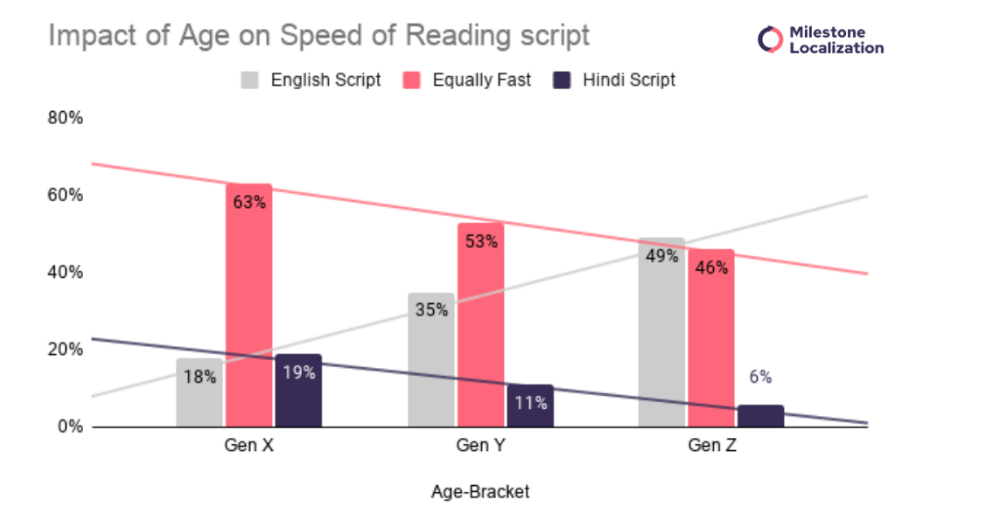
\includegraphics[width=0.8\textwidth]{plots/age_faster_read.png}
\end{figure}

From the above plot we can see that the people who are in the age group Gen Z are very less acquainted with the Hindi script. They mostly prefer to read it through the Latin script. They are more familiar wiht the English script one of the reasons being that most or the edication is nowadays done in the English language. Whereas in the older generation, as the education was in both Hindi and English, they are able to readd both of them equally fast. 

\subsubsection{Preferred Script}

\begin{figure}[H]
    \centering
    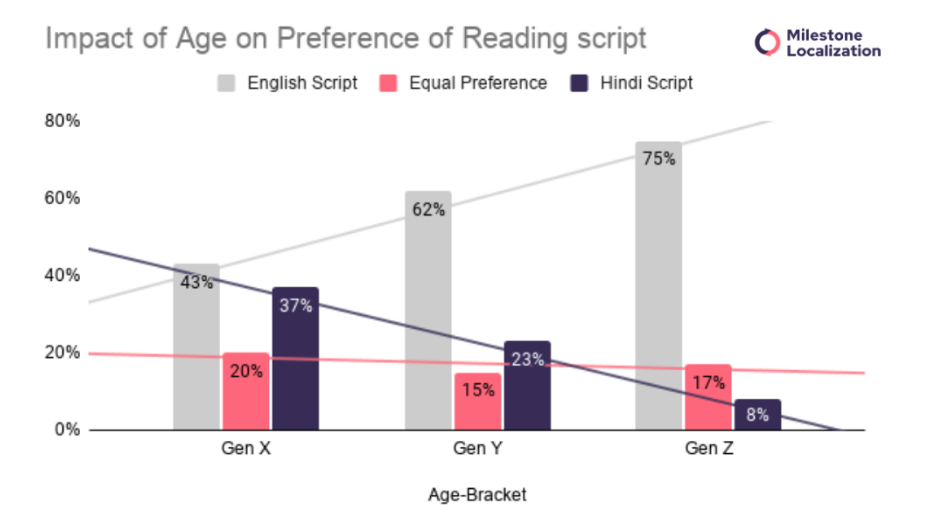
\includegraphics[width=0.8\textwidth]{plots/age_preferred_script.png}
\end{figure}

\subsubsection{Exposure to Hinglish}

\begin{figure}[H]
    \centering
    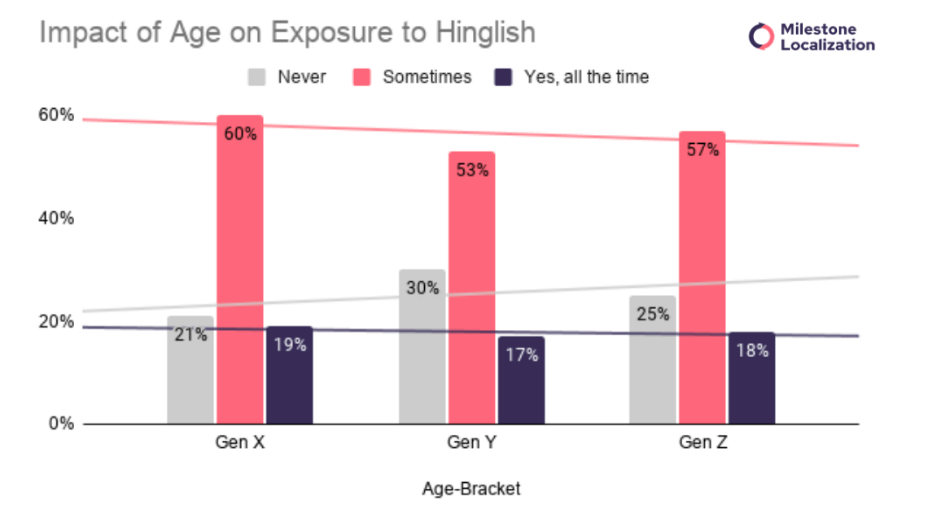
\includegraphics[width=0.8\textwidth]{plots/age_exposure.png}
\end{figure}

\subsection{Origin Factors}

\begin{figure}[H]
    \centering
    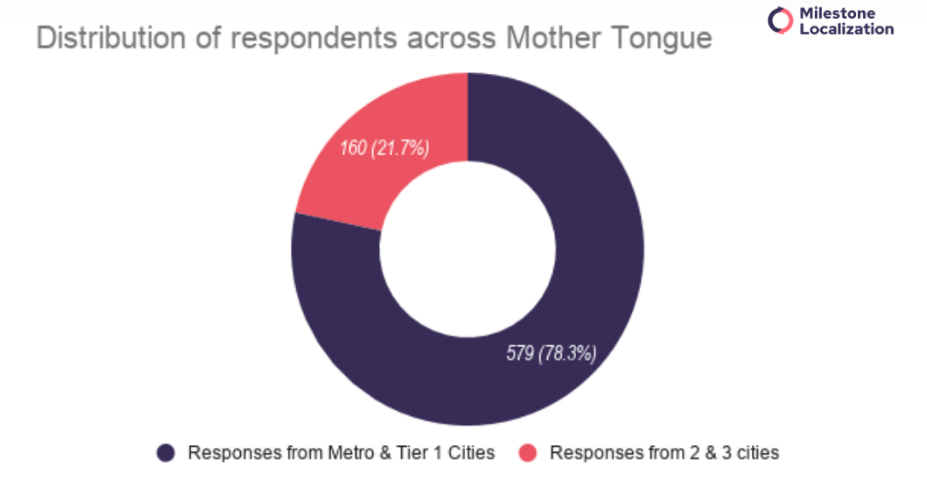
\includegraphics[width=0.8\textwidth]{plots/distribution_with_city.png}
\end{figure}

\subsubsection{Mixing of Languages}

\begin{figure}[H]
    \centering
    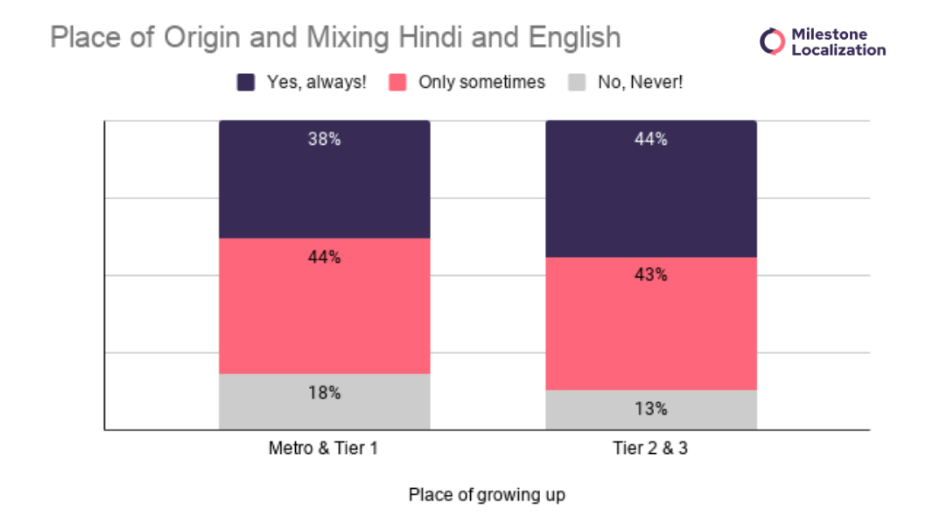
\includegraphics[width=0.8\textwidth]{plots/origin_mixing_language.png}
\end{figure}

\subsubsection{Speed of Reading}

\begin{figure}[H]
    \centering
    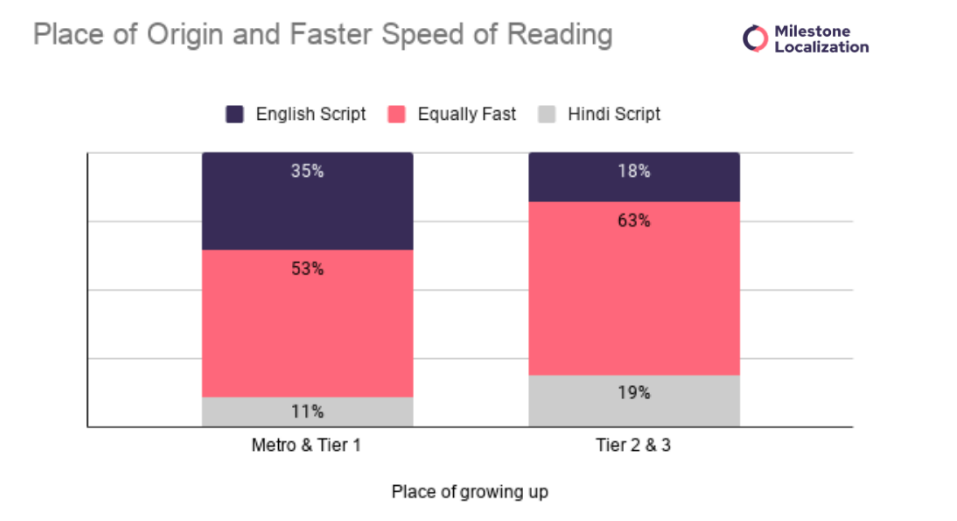
\includegraphics[width=0.8\textwidth]{plots/origin_faster_read.png}
\end{figure}

\subsubsection{Preferred Script}

\begin{figure}[H]
    \centering
    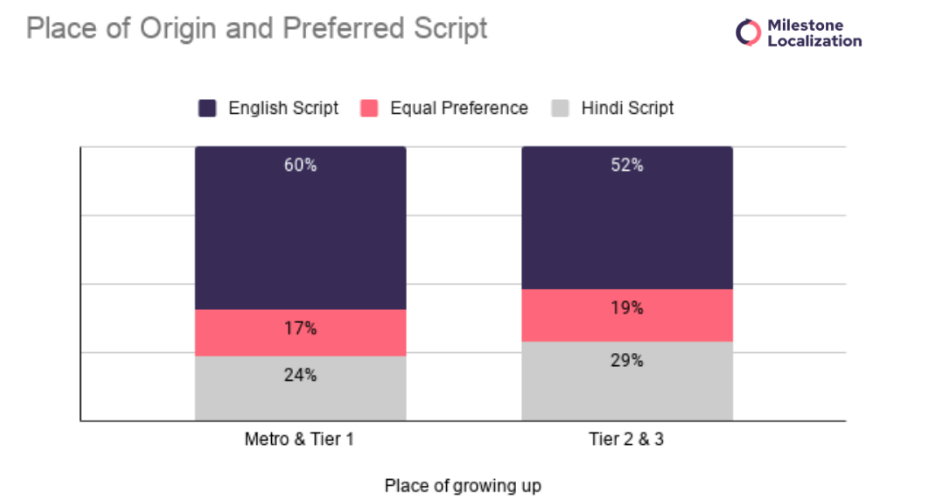
\includegraphics[width=0.8\textwidth]{plots/origin_preferred_script.png}
\end{figure}

\subsubsection{Exposure to Hinglish}

\subsection{Impact of Mother Tongue}

\subsubsection{Mixing of Languages}

\begin{figure}[H]
    \centering
    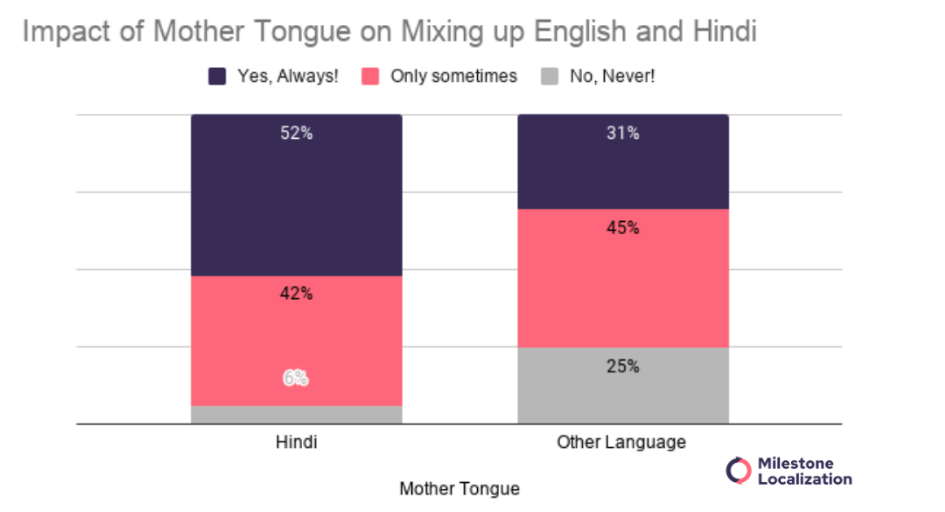
\includegraphics[width=0.8\textwidth]{plots/mother_mixing_language.png}
\end{figure}

\subsubsection{Speed of Reading}

\begin{figure}[H]
    \centering
    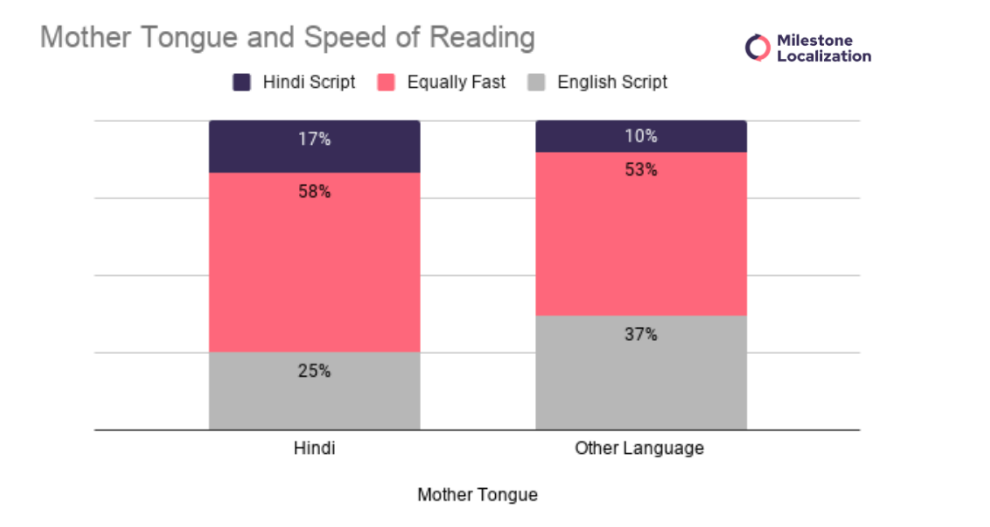
\includegraphics[width=0.8\textwidth]{plots/mother_faster_read.png}
\end{figure}

\subsubsection{Preferred Script}

\begin{figure}[H]
    \centering
    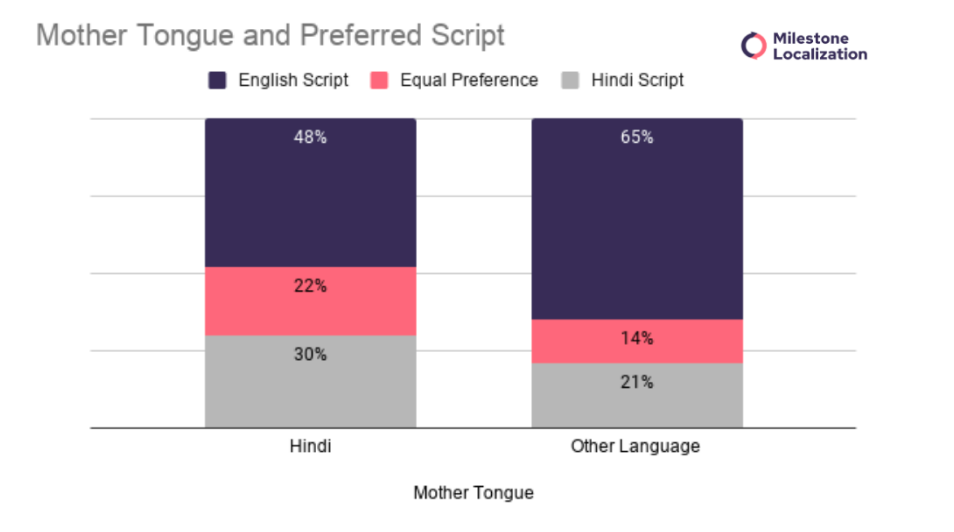
\includegraphics[width=0.8\textwidth]{plots/mother_preferred_script.png}
\end{figure}


\subsubsection{Exposure to Hinglish}

\begin{figure}[H]
    \centering
    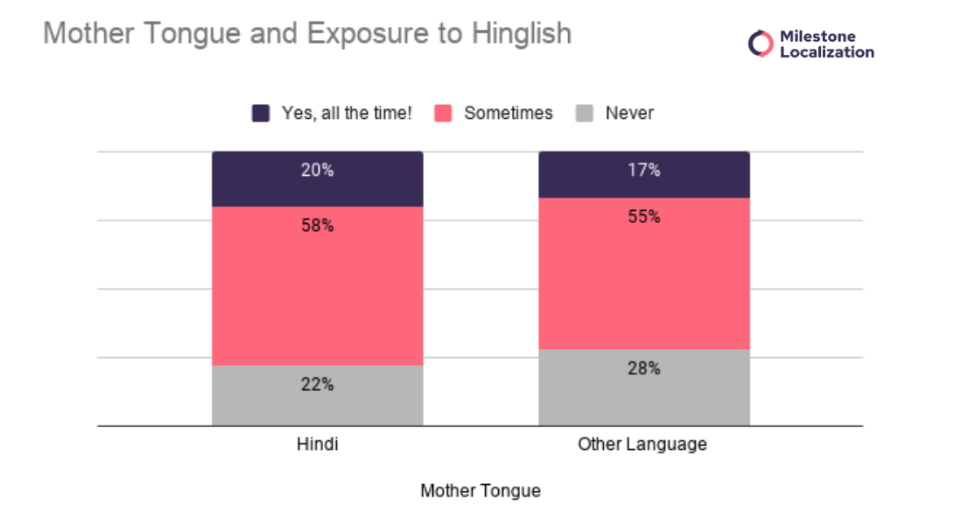
\includegraphics[width=0.8\textwidth]{plots/mother_exposure.png}
\end{figure}


\subsection{Frequent Usage}

\subsubsection{Mixing of Languages}

\begin{figure}[H]
    \centering
    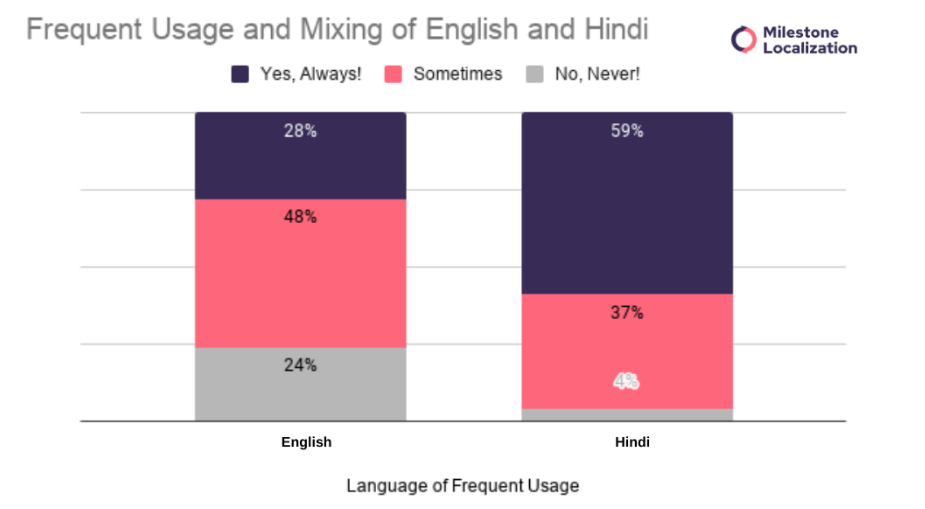
\includegraphics[width=0.8\textwidth]{plots/frequent_mixing_language.png}
\end{figure}

\subsubsection{Speed of Reading}

\begin{figure}[H]
    \centering
    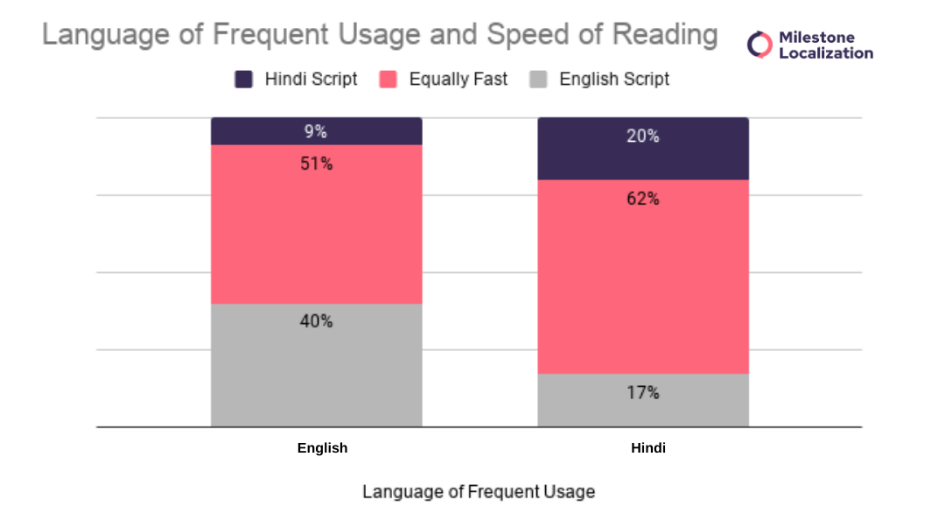
\includegraphics[width=0.8\textwidth]{plots/frequent_faster_read.png}
\end{figure}

\subsubsection{Preferred Script}

\begin{figure}[H]
    \centering
    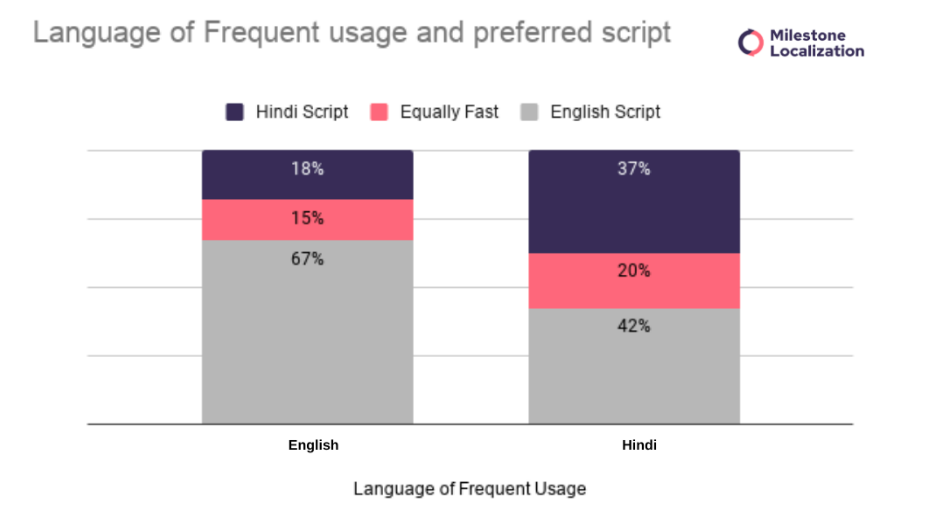
\includegraphics[width=0.8\textwidth]{plots/frequent_preferred_script.png}
\end{figure}

\subsubsection{Exposure to Hinglish}

\begin{figure}[H]
    \centering
    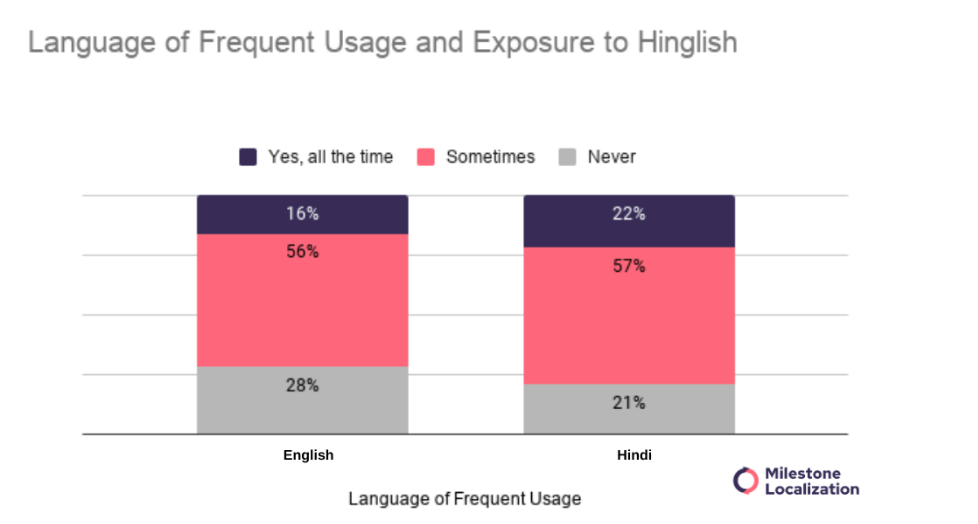
\includegraphics[width=0.8\textwidth]{plots/frequent_exposure.png}
\end{figure}

\section{Impact on Hindi and English}


\section{Conclusions}

\section{Notes and References}

\end{document}